\IfFileExists{SUBMIT}{
\documentclass[sigconf,review,anonymous]{acmart}
}{
\documentclass[sigconf,anonymous]{acmart}
}

\newcommand{\mytitle}{Input Debugging via Rich %and Fast 
Failure Feedback}
\renewcommand{\mytitle}{Repairing Inputs}


\usepackage{xspace}
\usepackage{array,multirow,graphicx}
\usepackage{float}
\usepackage{framed}
\usepackage{tikz,pgfplots,pgfplotstable}
\usetikzlibrary{calc,positioning,patterns}
\usepackage{hyperref}
\usepackage{cleveref}
\usepackage{boxedminipage}
\usepackage[inline]{enumitem}
\setlength{\FrameSep}{3pt}
\setlength{\OuterFrameSep}{2pt}
\newenvironment{result}{\begin{framed}\centering\it}{\end{framed}}

%% Identifiers
\def\|#1|{\textit{#1}}
\def\<#1>{\texttt{#1}}

\newcounter{todocounter}
\newcommand{\todo}[1]{\marginpar{$|$}\textcolor{red}{\stepcounter{todocounter}\footnote[\thetodocounter]{\textcolor{red}{\textbf{TODO }}\textit{#1}}}}
%\newcommand{\repl}[2]{\textcolor{red}{\textbf{REPLACE }\st{#1} \textit{#2}}}
%\newcommand{\rem}[1]{\textcolor{red}{\textbf{REMOVED }\st{#1}}}
\newcommand{\done}[1]{\marginpar{$*$}\textcolor{green}{\stepcounter{todocounter}\footnote[\thetodocounter]{\textcolor{black}{\textbf{DONE }}\textit{#1}}}}

% \newcommand{\todo}[1]{\textcolor{red}{\textbf{TODO: }\emph{#1}}}
% \newcommand{\com}[1]{\textcolor{orange}{\textbf{COMMENT: }\emph{#1}}}
\newcommand{\recheck}[1]{\textcolor{red}{#1}}
\newcommand{\revise}[1]{\textcolor{blue}{#1}}

\renewcommand{\done}[1]{} % comment to see responses.

\IfFileExists{SUBMIT}{
\renewcommand{\todo}[1]{}
\renewcommand{\done}[1]{}
%\renewcommand{\rem}[1]{}
%\renewcommand{\theendnotes}{}
}{
}

%--

% Own commands
\newcommand{\dd}{\textit{dd}\xspace}
\newcommand{\ddmin}{\textit{ddmin}\xspace}
%\newcommand{\ddmax}{\textit{ddmax}\xspace}
\newcommand{\test}{\textit{test}\xspace}
%\newcommand{\ddmaxg}{\textit{syntactic ddmax}\xspace}

\usepackage{pifont}
\newcommand{\pass}{\text{\ding{52}}\xspace}
\newcommand{\fail}{\text{\ding{56}}\xspace}
% \newcommand{\unresolved}{\textbf{?}}
\newcommand{\unresolved}{\lower0.1ex\hbox{\includegraphics*[height=1.7ex]{question.pdf}}}


\newcommand{\cpass}{{c_{\scriptscriptstyle \pass}}}
\newcommand{\cfail}{{c_{\scriptscriptstyle \fail}}}
\newcommand{\dpass}{{c'_{\scriptscriptstyle \pass}}}
\newcommand{\dfail}{{c'_{\scriptscriptstyle \fail}}}

%--

\newcommand{\approach}{\textsc{BRepair}\xspace}
\def\bfr{bFuzzerRepairer\xspace}
\def\ddmin{DDMin\xspace}
\newcommand{\ddmax}{\textit{DDMax}\xspace}
\newcommand{\ddmaxg}{\textit{DDmaxG}\xspace}
\newcommand{\bsimple}{\textit{bsimple}\xspace}
\newcommand{\brepair}{\textit{brepair}\xspace}

\tikzset{inlinenode/.style={draw=white,text=black,fill=light-gray,inner sep=.1em,outer sep=0em}}
\newcommand{\inlinenode}[1]{\text{\hspace{.1em}\tikz[baseline=(n.base)]{\node[inlinenode] (n) {\strut \hspace*{.3em}#1\hspace*{.3em}};}\hspace{.1em}}}
\newcommand{\inlinetext}[1]{\text{\hspace{.1em}\tikz[baseline=(n.base)]{\node[inlinenode] (n) {\strut \hspace*{.3em}\letterboxed{#1}\hspace*{.3em}};}\hspace{.1em}}}
\newcommand*\circled[1]{\tikz[baseline=(char.base)]{
            \node[shape=circle,draw,inner sep=0.3pt] (char) {#1};}}

\tikzset{%
simpletext/.style={draw=none,text=black,font=\normalfont\normalsize,align=center},
gparsetreenode/.style={minimum width=6mm,minimum height=5mm},
lparsetreenode/.style={gparsetreenode,simpletext,rectangle,draw=white,fill=white,align=center},
lparsetreeerrornode/.style={lparsetreenode,font=\bfseries},
lparsetreephantomnode/.style={gparsetreenode,edge from parent/.append style={draw=none},shape=coordinate,minimum width=15mm},
lparsetreestrikethrough/.style={draw=black,thick},
lparsetreedeletednode/.style={lparsetreenode,append after command={\pgfextra \draw[lparsetreestrikethrough] (\tikzlastnode.north west) -- (\tikzlastnode.south east); \draw[lparsetreestrikethrough] (\tikzlastnode.north east) -- (\tikzlastnode.south west);\endpgfextra}},
lparsetree/.style={node distance=5mm,level distance=10mm,every node/.style={lparsetreenode},edge from parent/.style={draw=black,-latex,shorten >=.5mm}
},
lflowchartnode/.style={lparsetreenode,draw=black,rounded corners=.5pt},
blockdiagramlines/.style={draw,stroke=black,line width=1.2pt},
blockdiagramarrow/.style={blockdiagramlines,->},
blockdiagramdashedarrow/.style={blockdiagramarrow,dashed},
blockdiagramannot/.style={blockdiagramlines,text=black,align=center},
blockdiagramblock/.style={lflowchartnode,blockdiagramannot,minimum width=1.5cm,minimum height=0.5cm,text width=1.9cm},
blockdiagrammicroblock/.style={blockdiagramannot,font=\tiny,minimum width=1.5cm,minimum height=.5cm,rounded corners=.5pt},
blockdiagramarrowcaption/.style={font=\scriptsize\sffamily,inner sep=1.5pt,text=black},
blockdiagramouterbox/.style={blockdiagramlines,densely dotted,line width=.7pt},
blockdiagramouterboxcaption/.style={blockdiagramarrowcaption,font=\itshape\scriptsize,inner sep=1pt},
pics/numbering/.style args={#1}{code={
    \node[draw=black,shape=circle,fill=white,text=black,font=\ttfamily\scriptsize,inner sep=1pt,text width=8pt,align=center,outer sep=0] (-number) {#1};
}}}

% Boxes around letters
\definecolor{light-gray}{gray}{0.87}
\makeatletter
\newcommand\letterboxed[1]{%
\setlength{\fboxsep}{0pt}%
  \@tfor\@ii:=#1\do{%
    \fcolorbox{white}{light-gray}{\texttt{\strut\@ii}}%
  }%
}
\makeatother


%%
%% \BibTeX command to typeset BibTeX logo in the docs
\AtBeginDocument{%
  \providecommand\BibTeX{{%
    \normalfont B\kern-0.5em{\scshape i\kern-0.25em b}\kern-0.8em\TeX}}}

%% Rights management information.  This information is sent to you
%% when you complete the rights form.  These commands have SAMPLE
%% values in them; it is your responsibility as an author to replace
%% the commands and values with those provided to you when you
%% complete the rights form.
\setcopyright{acmcopyright}
\copyrightyear{2018}
\acmYear{2018}
\acmDOI{XXXXXXX.XXXXXXX}

%% These commands are for a PROCEEDINGS abstract or paper.
\acmConference[ESEC/FSE 2022]{The 30th ACM Joint European Software Engineering Conference and Symposium on the Foundations of Software Engineering}{14 - 18 November, 2022}{Singapore}
\acmPrice{15.00}
\acmISBN{978-1-4503-XXXX-X/18/06}

\usepackage[utf8]{inputenc}

\begin{document}

\title{\mytitle}

\author{Ben Trovato}
\authornote{Both authors contributed equally to this research.}
\email{trovato@corporation.com}
\orcid{1234-5678-9012}
\author{G.K.M. Tobin}
\authornotemark[1]
\email{webmaster@marysville-ohio.com}
\affiliation{%
  \institution{Institute for Clarity in Documentation}
  \streetaddress{P.O. Box 1212}
  \city{Dublin}
  \state{Ohio}
  \country{USA}
  \postcode{43017-6221}
}

\author{Lars Th{\o}rv{\"a}ld}
\affiliation{%
  \institution{The Th{\o}rv{\"a}ld Group}
  \streetaddress{1 Th{\o}rv{\"a}ld Circle}
  \city{Hekla}
  \country{Iceland}}
\email{larst@affiliation.org}

\author{Valerie B\'eranger}
\affiliation{%
  \institution{Inria Paris-Rocquencourt}
  \city{Rocquencourt}
  \country{France}
}

\author{Aparna Patel}
\affiliation{%
 \institution{Rajiv Gandhi University}
 \streetaddress{Rono-Hills}
 \city{Doimukh}
 \state{Arunachal Pradesh}
 \country{India}}

\author{Huifen Chan}
\affiliation{%
  \institution{Tsinghua University}
  \streetaddress{30 Shuangqing Rd}
  \city{Haidian Qu}
  \state{Beijing Shi}
  \country{China}}

\author{Charles Palmer}
\affiliation{%
  \institution{Palmer Research Laboratories}
  \streetaddress{8600 Datapoint Drive}
  \city{San Antonio}
  \state{Texas}
  \country{USA}
  \postcode{78229}}
\email{cpalmer@prl.com}

\author{John Smith}
\affiliation{%
  \institution{The Th{\o}rv{\"a}ld Group}
  \streetaddress{1 Th{\o}rv{\"a}ld Circle}
  \city{Hekla}
  \country{Iceland}}
\email{jsmith@affiliation.org}

\author{Julius P. Kumquat}
\affiliation{%
  \institution{The Kumquat Consortium}
  \city{New York}
  \country{USA}}
\email{jpkumquat@consortium.net}

%%
%% By default, the full list of authors will be used in the page
%% headers. Often, this list is too long, and will overlap
%% other information printed in the page headers. This command allows
%% the author to define a more concise list
%% of authors' names for this purpose.
\renewcommand{\shortauthors}{Trovato and Tobin, et al.}

\date{February 2022}

\begin{abstract}
Data cleansing and data repair are some of the most developer time intensive
tasks in many fields that aggregate data from multiple resources. In many cases,
the data may be entered by hand, and while ostensibly conforming to a given
format, is often unparsable by machines.
In such cases, a data engineer has to manually repair the corrupt data such that
it follows a given format, and hence processable by the next program.
Such manual repair can be time consuming, and error-prone.

In this work, we show that incorporating light-weight error-feedback to parsers
is sufficient to repair any corrupt input string with maximal closeness to the
semantics of input data.

Given a conforming program, and any corrupt input, \approach provides a set
of repairs prioritized by the distance of the repair from the original input.

We show that our approach can remove the limitations inherent in \ddmax, the
previously best known approach, both in terms of what it can repair, as well as
in terms of the set of repairs offered. In our evaluation of \approach, we found
that it can outperform \ddmax in input repair, and can repair all input corruptions
that were induced.
\end{abstract}

% \begin{abstract}
% %Problem/
% %\textbf{Context:} 
% %\revise{
% Program failures are sometimes induced by %when 
% \textit{faulty inputs}, rather than \textit{buggy programs}, % are fed to \textit{valid} programs, 
% e.g., 
% %This can be 
% due to incomplete or corrupted data. When an input \textit{solely} %is responsible for the program 
% induces a failure in a valid program, the developer is saddled with the task of 
% \textit{input debugging}.  %}
% %\textbf{Objective:}  
% %\revise{
% Debugging \textit{failure-inducing inputs} involves identifying the  \textit{root cause} of the failure (e.g., the faulty input fragment)
% % causing the failure), 
% and \textit{repairing the input} such that it can be processed by the program. This is particularly difficult for structured inputs with complex input specifications (e.g., JSON).  
% %} 
% %\textbf{Methodology:} 
% %\revise{
% In this work, we present a \textit{language-agnostic, black-box} testing approach (called \approach) that leverages 
% %ich and fast 
% \textit{failure feedback} %from the program 
% to automatically debug faulty inputs. The key insight of our approach %(called \approach) 
% is to \textit{semantically} repair faulty inputs 
% %to debug inputs via %by employing %a 
% %combination of 
% %\textit{test experimentation} that leverages 
% using %leverage 
% the richness of %and speed of 
% \textit{failure feedback}, %to \textit{semantically}, 
% such as 
% %Specifically, \approach uses program feedback to 
% %%. \approach employs  to identify %ing input properties such as the 
% %identify 
% the \textit{validity, incompleteness and incorrectness} checks of input fragments. 
% Given a failure-inducing input and a valid program,  
% \approach performs %conducts %test experiments 
% semantic checks of input subsets to identify %ies 
% faulty input fragments. 
% %by conducting semantic checks of input fragments (e.g., (in)completeness) using test experiments. 
% It then repairs the faulty input by removing or \textit{synthesizing} candidate input elements. % for repair.  
% \revise{In our evaluation, \todo{\approach repaired ... recovered  ...} 
% In addition, \approach overcomes the span length issue of (lexical) DDmax and outperforms DDMax by X\%, %despite %   %} In addition, \approach addresses several limitations of the state of the art, e.g., it overcomes the span length issue of (lexicial) DDmax and it does 
% without access to an input grammar (syntactic DDmax). }
% 
% %\textbf{Conclusion:}
% 
% 
% \end{abstract}

%%
%% The code below is generated by the tool at http://dl.acm.org/ccs.cfm.
%% Please copy and paste the code instead of the example below.
%%
% \begin{CCSXML}
% <ccs2012>
%  <concept>
%   <concept_id>10010520.10010553.10010562</concept_id>
%   <concept_desc>Computer systems organization~Embedded systems</concept_desc>
%   <concept_significance>500</concept_significance>
%  </concept>
%  <concept>
%   <concept_id>10010520.10010575.10010755</concept_id>
%   <concept_desc>Computer systems organization~Redundancy</concept_desc>
%   <concept_significance>300</concept_significance>
%  </concept>
%  <concept>
%   <concept_id>10010520.10010553.10010554</concept_id>
%   <concept_desc>Computer systems organization~Robotics</concept_desc>
%   <concept_significance>100</concept_significance>
%  </concept>
%  <concept>
%   <concept_id>10003033.10003083.10003095</concept_id>
%   <concept_desc>Networks~Network reliability</concept_desc>
%   <concept_significance>100</concept_significance>
%  </concept>
% </ccs2012>
% \end{CCSXML}

% \ccsdesc[500]{Computer systems organization~Embedded systems}
% \ccsdesc[300]{Computer systems organization~Redundancy}
% \ccsdesc{Computer systems organization~Robotics}
% \ccsdesc[100]{Networks~Network reliability}

%%
%% Keywords. The author(s) should pick words that accurately describe
%% the work being presented. Separate the keywords with commas.
\keywords{input debugging, input repair, parse failures, structured inputs}


%% A "teaser" image appears between the author and affiliation
%% information and the body of the document, and typically spans the
%% page.
% \begin{teaserfigure}
%   \includegraphics[width=\textwidth]{sampleteaser}
%   \caption{Seattle Mariners at Spring Training, 2010.}
%   \Description{Enjoying the baseball game from the third-base
%   seats. Ichiro Suzuki preparing to bat.}
%   \label{fig:teaser}
% \end{teaserfigure}

%%
%% This command processes the author and affiliation and title
%% information and builds the first part of the formatted document.
\maketitle

\section{Introduction}

Data, especially from external, often human sources need to be collected and
aggregated before information processing algorithms can be run on it to extract
insights. Unfortunately, not every source may agree on the format specification.
For example, (1)~there are numerous JSON libraries with slightly different
definitions of what the JSON format is~\cite{harrand2021behavioral,seriot2016parsing}.
(2)~there are numerous database systems, each supporting a slightly
different SQL format~\cite{arvin2018comparison}, (3)~a variety of markdown
syntaxes with subtle differences~\cite{visnoviz2019comparison}, and (4)~various
\<C> compilers each supporting a slightly different interpretation of the \<C> language.
That is, it is often impossible to process an artifact that was generated with
a different implementation in mind. Another issue is that many such artifacts
are created by hand, and the process of manual generation can be error-prone.

Given such artifacts that are \emph{almost} but \emph{not quite} parsable,
consuming such resources, and aggregating them often involves trying to
maximally parse them by minimizing parse errors~\cite{kirschner2020debugging}.
If the parser at hand conforms to a formal specification such as a context-free
grammar, and this grammar is available,
%context-free grammar, and an acceptable formal grammar is available,
the challenge of repairing the input and making it parsable can be solved using
\emph{error-correcting} parsers~\cite{aho1972minimum,diekmann2020dont}.
The idea in such parsers is to generate a universal grammar that captures
any mutation of the base grammar. Any parse of the input string that employs a
mutation is penalized, and the parse with minimal mutation is chosen as the
best parse, and the corresponding mutation the best repair. The limitation of
this approach is that it assumes the existence of a formal grammar in the first
place, which completely captures the intended structure.
However, formats such as markdown~\cite{gruber2004markdown} does not have
a formal grammar; Documents in languages such as \<C> can contain semantic
information that is not captured in the contex-free grammar, and may not be
discardable. Finally, even when the base grammar is context-free grammar (as in
the case of JSON) the serializer and deserializer may implement common subsets
beyond the base grammar (e.g comments and unquoted keys in JSON) which may
contain important information. Hence, relying on error-correcting parsers may
be unoptimal for fixing error corruption.

In circumstances where one can't rely on a base grammar, the only option so far
has been \ddmax~\cite{kirschner2020debugging}. The \ddmax works similar to
delta-debugging~\cite{zeller2002simplifying}, but in reverse. The idea
is that given a corrupt input which induces a parse error, and a way to
decompose the input into independent fragments (called deltas), one can
successively minimize the parse-error inducing part of the input resulting in a
maximal parsing input.

\begin{table*}\centering
\footnotesize
\caption{\ddmax limitations}
\begin{tabular}{|l | c | c | l |}
\hline
Example & \ddmax repair & \approach repair & \ddmax limitation \\
\hline
\letterboxed{\{\ "item":\ "Apple",\ "price":\ ***3.45\}} & \letterboxed{\ \ \ \
3.45} & \letterboxed{\{\ "item":\ "Apple",\ "price":\ 3.45\}} & Rich structure
(spans) \\
\letterboxed{\{\"ABCD":[*"1,2,3,4,5,6"]*\}} & 
\letterboxed{123456} & 
\letterboxed{\{\"ABCD":["1,2,3,4,5,6"]\}} & 
Rich Structure (multiple-faults) \\
\letterboxed{\{\ "name":\ "Dave"\ "age":\ 42\ \}} &
\letterboxed{\{\ "name":\ "Daveage":\ 42\ \}} &
\letterboxed{\{\ "name":\ "Dave",\ "age":\ 42\ \}} &
Limited repair options (deletion) \\
\hline
\end{tabular}
\label{tab:ddmaxlimitations}
%\vspace{-0.5cm}
\end{table*}

\ddmax works very well for most inputs. However, it has two major limitations
(1)~Limitations due to rich input structure,
(2)~limited repair options available.
We show examples of each in \Cref{tab:ddmaxlimitations}.

The essential limitation is that \ddmax is modeled after \ddmin, where one of
the unstated assumptions is that the $\delta$ fragments that are non
contributing to the failure observed can be independently removed without
affecting the failure observed. When this assumption is not met, (i.e. where
the inputs have a rich structure) the minimal fragment produced by \ddmin
can be suboptimal.

Our \brepair algorithm starts with the corrupted input and quickly finds the
maximal parsable prefix using a binary search.
For example, in \Cref{fig:bad-json-input}, \brepair finds the maximal parsable
prefix to be \letterboxed{\{\ "name":\ "Dave"\ }, and the boundary happens
at \\
\letterboxed{\{\ "name":\ "Dave"\ "} where the parser response shifts from
\emph{incomplete} to \emph{incorrect}.
At this point, \brepair applies deletion, or insertion of characters
in order. In this case, the \<"> is deleted first, and the
resulting input \\
\letterboxed{\{\ "name":\ "Dave"\ age":\ 42 \}} is checked to
see if it resulted in increasing the size of the maximum parsable prefix. Here,
we see that the maximal parse boundary remains the same. Hence \brepair next
attempts to insert a character. There are 128 printable characters in ASCII,
out of which, only space characters and comma (\<,>) can be inserted here,
resulting in an increase of maximal parse prefix. Out of this, comma
results in the maximum advancement of the parse boundary, resulting in the
newly constructed string: \\
\letterboxed{\{\ "name":\ "Dave"\ ,\"age":\ 42\ \}}
which is accepted as a valid repair.

%---
% Example for Span Problem
%---
\begin{figure}
\begin{center}
\letterboxed{\{\ "item":\ "Apple",\ "price":\ ***3.45\ \}}
\end{center}
%\vspace{-0.6\baselineskip}
  \caption{\ddmax repairs this JSON to \mbox{``\<\ \ \ \ 3.45>''}}
   %\Cref{fig:bad-json-input-asterisks}. This is very
%similar to Kirchner et al.~\cite[Figure 1]{kirschner2020debugging} 
\label{fig:bad-json-input-asterisks}

\end{figure}

\subsection{Limitations due to rich input structure}
One of the major problems with \ddmax is that it can fail when certain
corruption patterns are encountered din the input string.

As an example, consider the fragment \letterboxed{[*+]}.
Here, the JSON string is invalid because it contains two invalid characters.
The operation of \ddmax (\Cref{fig:ddmax}) is as follows:

\begin{enumerate}
\item The operation starts with $\ddmax_2(\emptyset, 2)$
\item  $|\cfail - \emptyset| \ne 1$. Hence, the base case does not apply
\item Increase to complement:\\
$\cfail - \Delta_2$= \letterboxed{+]} \fail \\
$\cfail - \Delta_2$= \letterboxed{[*} \fail \\
\item Increase to subset:\\
$\cfail \cup \Delta_1$=\letterboxed{[*} \fail \\
$\cfail \cup \Delta_2$= \letterboxed{+]} \fail \\
\item Increase grannularity: $n < |\cfail-\dpass|$ which is $2 < |\cfail-\emptyset|$ \pass \\
  Hence the next iteration is:
  $\ddmax_2\bigl(\emptyset, 4)\bigr) $
\item  $|\cfail - \emptyset| \ne 1$. Hence, the base case does not apply.
\item Increase to complement:\\
$\cfail - \Delta_2$= \letterboxed{*+]} \fail \\
$\cfail - \Delta_2$= \letterboxed{[+]} \fail \\
$\cfail - \Delta_2$= \letterboxed{[*]} \fail \\
$\cfail - \Delta_2$= \letterboxed{[*+} \fail \\
\item Increase to subset:\\
$\cfail \cup \Delta_1$=\letterboxed{[} \fail \\
$\cfail \cup \Delta_1$=\letterboxed{*} \fail \\
$\cfail \cup \Delta_1$=\letterboxed{+} \fail \\
$\cfail \cup \Delta_1$=\letterboxed{]} \fail \\
\item Increase to grannularity: $4 < 4$ \fail\\
\item The solution is $\emptyset$.
\end{enumerate}

That is, this particular invalid JSON string can't be repaired by \ddmax.
While this may seem like not much of information loss, consider
\Cref{fig:bad-json-input-asterisks} which is similar to
Kirchner et al.~\cite[Figure 1]{kirschner2020debugging} but with an extra
\letterboxed{*}. This results in a repair of \mbox{``\<\ \ \ \ 3.45>''},
resulting in information loss.

One of the issues here is that unlike \ddmin, \ddmax can't require independence
of $\Delta$ sequences. That is, \ddmin requires that each non-failure causing
fragment can be independently removed without impacting the failure. An
equivalent condition for \ddmax would be that one can add each non-failure
causing fragment to the passing input independently. However, this fails
when we have rich input structure as illustrated by the above example.
Of course, onece the input processor conforms to this constraint, \ddmax will
have no problems maximizing any inputs. However, this can be a rather strong
constraint in practice.

\subsection{Limitations due to multiple faults}
\todo{I think that all these issues with \ddmax has one single cause -- the
rich input structure. I have mentioned it above. Perhaps we should simply
consolidate all into one.}
Another issue (acknowledged by the \ddmax paper) is that multiple errors and
multiple repairs can be a limitation. \ddmax paper claims that ``when given
inputs with multiple errors, \ddmax will produce an input that repairs all of
them. However, if theere are multiple ways to repair the input, \ddmax will
produce only one''. The problem is that, \ddmax's choice need not be optimal.
For example, consider \Cref{fig:bad-json-input2}. \ddmax repairs this input
to \<123456> which loses the structure as well as changes the type from
\<string> to \<number>. Hence, \ddmax can't repair inputs with multiple faults
effectively.

%One of the ambiguities here is that it is not immediately
%clear what a repair means. For example the empty set $\emptyset$ is assumed to
%be passing. Hence, is $\emptyset$ a valid repair?

\begin{figure}
\begin{center}
\letterboxed{\{\"ABCD":[*"1,2,3,4,5,6"]*\}}
\end{center}
%\vspace{-0.6\baselineskip}
\caption{\ddmax repairs this JSON to ``\<123456>''}
\label{fig:bad-json-input2}
\end{figure}

\begin{figure}
\begin{center}
\letterboxed{\{\ "name":\ "Daveage"\ \}}
\end{center}
%\vspace{-0.6\baselineskip}
\caption{Failing input repaired with DDMax}
\label{fig:bad-json-input-ddmax}
\end{figure}

\subsection{Limited Options for Repair}
The second major limitation of
\ddmax is that the only operation in its toolbox is \emph{deletion} of input
fragments. Consider \Cref{fig:bad-json-input}.
%\Cref{fig:bad-json-deletion}.
%\begin{figure}
%\begin{center}
%\letterboxed{\{\ "fruits:\ ["Apple",\ "Orange",\ "Banana"]\}}
%\end{center}
%%\vspace{-0.6\baselineskip}
%\caption{Invalid JSON with non-optimal repair by \ddmax}
%\label{fig:bad-json-deletion}
%\end{figure}
%---
% Example for Insertion
%---
\begin{figure}
\begin{center}
\letterboxed{\{\ "name":\ "Dave"\ "age":\ 42\ \}}
\end{center}
%\vspace{-0.6\baselineskip}
\caption{Failing JSON input}
\label{fig:bad-json-input}
\end{figure}
\begin{figure}
\begin{center}
\letterboxed{\{\ "name":\ "Daveage"\ \}}
\end{center}
%\vspace{-0.6\baselineskip}
\caption{Failing input repaired with DDMax}
\label{fig:bad-json-input-ddmax}
\end{figure}
Here, there is a missing quote in the key. \ddmax repair of this string will
result in \Cref{fig:bad-json-input-ddmax}. The problem is that, deletion of
fragments alone can lead to significant corruption of information.

% A problem of DDMax is that it only supports deleting parts of the file under test while repairing the file.
%Especially for highly-structured input formats like the JSON file seen in \Cref{fig:bad-json-input}, it is often the case that by inserting a simple character in the file, more information can be recovered in the file than by just deleting characters.

%--

%One example for such an algorithm that localizes faults in failure-inducing inputs is \emph{Delta-Debugging}~\cite{zeller2002simplifying}.
%It minimizes an input that induces a failure in a subject program while the minimized inputs still trigger the same bug.
%In a similar manner, \emph{DDMax}~\cite{kirschner2020debugging} is a modification of the Delta-Debugging algorithm that, instead of minimizing test cases, maximizes failure-inducing input files while not triggering failures in the subject program.
% The \emph{bFuzzer} algorithm~\cite{gopinath2020fuzzing} is an input generator that determines valid continuations for input prefixes by making use of rich failure feedback.
% The subject program does not only give feedback whether an input is accepted or not, but also whether the input is incorrect or incomplete.
% Based on this input generation algorithm, \bfr makes use of this rich failure feedback to allow both insertions and deletions at the fault location.
% 
% 
% %TODO ...
% Another problem occurring with DDMax is that it works very inefficient on inputs where the failure-inducing characters span a certain range in the file.% TODO which range?
% Consider the file shown in \Cref{fig:bad-json-input-asterisks} -- a JSON object where the number \letterboxed{3.45} is preceded by three asterisks, rendering the file corrupted.
% This example is similar to the one chosen in the introduction of \emph{Debugging Inputs}!\cite{kirschner2020debugging}.
% % 37 -> 18 -> 9 -> 4
% % { "item": "Apple", "price": ***3.45 }
% %                   ->
% %          ->       ->       ->
% %     ->  ->  ->  ->  ->  ->  ->  ->   
% When repairing this file, DDMax would first split the file in half, then in quarters and in eigths, finally trying to remove \letterboxed{***3} and \letterboxed{.45 \}}.
% Those attempts do not succeed, so it tries to remove \letterboxed{**} and \letterboxed{*3} which also fails.
% %TODO elaborate/rewrite?
% 
% With \bfr, repairing the file results in the file seen in \Cref{fig:bad-json-input-repaired-asterisks} -- \bfr first detects the fauklt to be at the leftmost asterisk.
% It then tries to insert characters (a \letterboxed{"} and a \letterboxed{ } which are both valid continuations of the prefix) and delete one asterisk.
% In the alternative where the \letterboxed{"} was inserted, \letterboxed{***3.45\ } can successfully be inserted from the original file.
% Then, \bfr tries both inserting the \letterboxed{\}} from the original file and another \letterboxed{"} which succeeds and results in the repaired file.
% 

This is, of course, not an ideal state of affairs. Unfortunately, \ddmax is
likely the best one can do unless one is willing to test all possible
subsequences of the input, which leads to combinatorial explosion. The main
issue here is that unlike with delta-debugging~\cite{zeller2002simplifying},
there is no real definition of progress. We do not know if 
\letterboxed{\{\ "A":\ *3\}} is better than
\letterboxed{\{\ "A":\ **3\}} or
\letterboxed{\{\ A":\ **3\}} because all three returns the same
result -- parse error.

All is, however, not lost. This paper shows that such corrupted inputs can
still be repaired adequately if the input processor can provide at least some
indication of progress. When given an input, we require the input
processor to indicate whether the input is merely incomplete -- that is, the
input is a prefix of a valid acceptable input -- or is incorrect -- that is, no
suffix to this input will result in a valid input.

This requirement is not hard to accomplish. In most cases, parsers already
provide precise information as to the point at which the parse failed, which
can be used directly in our algorithm. In the cases where parers do not provide
this information, obtaining this information by external instrumentation is
possible as demonstrated by Bj\"orn et al.~\cite{mathis2019parser}. If
the program is hard to instrument, adding failure feedback that we require is
not difficult~\cite{gopinath2020fuzzing}.

Our \brepair algorithm starts with the corrupted input and quickly finds the
maximal parsable prefix using a binary search.
For example, in \Cref{fig:bad-json-input}, \brepair finds the maximal parsable
prefix to be \letterboxed{\{\ "name":\ "Dave"\ }, and the boundary happens
at \\
\letterboxed{\{\ "name":\ "Dave"\ "} where the parser response shifts from
\emph{incomplete} to \emph{incorrect}.
At this point, \brepair applies deletion, or insertion of characters
in order. In this case, the \<"> is deleted first, and the
resulting input \\
\letterboxed{\{\ "name":\ "Dave"\ age":\ 42 \}} is checked to
see if it resulted in increasing the size of the maximum parsable prefix. Here,
we see that the maximal parse boundary remains the same. Hence \brepair next
attempts to insert a character. There are 128 printable characters in ASCII,
out of which, only space characters and comma (\<,>) can be inserted here,
resulting in an increase of maximal parse prefix. Out of this, comma
results in the maximum advancement of the parse boundary, resulting in the
newly constructed string: \\
\letterboxed{\{\ "name":\ "Dave"\ ,\"age":\ 42\ \}}
which is accepted as a valid repair.

In the case of \Cref{fig:bad-json-input-asterisks}, \brepair quickly finds the
first \<*> to be the parse boundary. At this point, deletion, or insertion
fails to advance the parse boundary. Indeed, there are no possible
insertion continuations found after \\
\letterboxed{\{\ "item":\ "Apple",\ "price":\ *}.\\
Hence, \brepair attempts two consecutive operations. Hence, since two
insertions is no longer possible, it attempts a deletion followed by insertion,
and two deletions. Deletion of a \<*> followed by insertion of \<"> does allow
the parse to proceed, resulting in \\
\letterboxed{\{\ "item":\ "Apple",\ "price":\ "**3.45\}}.\\
\emph{incomplete} with an unclosed quote, and a penalty of two. We also have
another thread with:
\letterboxed{\{\ "item":\ "Apple",\ "price":\ }\\
as the maximal parse boundary after deletions of two \<*> characters with the
same penalty. Since deletion is prioritized, we apply deletion on the second
thread where deletion is applicable, resulting in:\\
\letterboxed{\{\ "item":\ "Apple",\ "price":\ 3.45\}}.\\
Since the first thread does not complete with any change with a penalty of
three, we choose \\
\letterboxed{\{\ "item":\ "Apple",\ "price":\ 3.45\}}\\
as the solution.

%at which boundary the prefix shifts between incomplete and incorrect.
% It then iteratively applies
% deletion, insertion, and alteration of the character at the point of failure to
% find the least cost modification that would let the parse proceed further,
% generating a larger prefix. Proceeding in this fashion, the algorithm generates
% a set of plausible repairs ordered by their edit distance that can be used by
% the developer for fixing the input corruption.
% 
% In the example seen in \Cref{fig:bad-json-input-repaired}, \brepair first determines a valid (incomplete) prefix of the input file, i.e., \texttt{\{ "name": "Dave"}.
% It then tries to append characters such that the prefix stays valid - in this example, \letterboxed{\}} and \letterboxed{,} are tried to be inserted.
% Then, as much of the original file is appended to the prefix, until it becomes valid (and the rest of the original file is either appended, or deleted successively).
% This results in the final repaired file seen in \Cref{fig:bad-json-input-repaired}.
% \begin{figure}
% \begin{center}
% \letterboxed{\{\ "name":\ "Dave",\ "age":\ 42\ \}}
% \end{center}
% %\vspace{-0.6\baselineskip}
% \caption{Failing input repaired with \brepair}
% \label{fig:bad-json-input-repaired}
% \end{figure}
% \begin{figure}
% \begin{center}
% \letterboxed{,}
% \end{center}
% %\vspace{-0.6\baselineskip}
% \caption{Difference between failing and repaired input}
% \label{fig:bad-json-input-diff}
% \end{figure}
% \begin{figure}
% \begin{center}
% \letterboxed{\{\ "item":\ "Apple",\ "price":\ "***3.45\ "\}}
% \end{center}
% %\vspace{-0.6\baselineskip}
% \caption{Failing input repaired with \brepair}
% \label{fig:bad-json-input-repaired-asterisks}
% \end{figure}

\todo{
\textbf{note:} In the algorithm, we need to limit possible insertions.
Unconstrained insertions are possible only for two characters. If we
have constraints on the initial character, more insertions can be allowed,
until the choices reach a configurable number (e.g. 100,000)
beyond which deletion should take precedence.
}
\\
\noindent\textbf{Contributions.}
\begin{itemize}
  \item We identify one of the major limitations to \ddmax -- the limitation due to rich struture, which can be fixed only by requiring additional constraints.
  \item We provide two bug fixes to \ddmax.
  \item We propose \approach which does not have these limitations.
\end{itemize}
%TODO
\section{Overview}

\begin{figure*}[t]
\begin{boxedminipage}{\textwidth}
\smallskip
\ \begin{minipage}{0.9\textwidth}
\subsection*{Maximizing Delta Debugging Algorithm}
\medskip

Let $\test$ and $\cfail$ be given such that $\test(\emptyset) = \pass \land
\test(\cfail) = \fail$ hold.

The goal is to find $\dpass = \ddmax(\cfail)$ such that $\dpass \subset \cfail$, $\test(\dpass) = \pass$, and~$\Delta = \cfail - \dpass$ is 1-minimal.

The \emph{maximizing Delta Debugging algorithm} $\ddmax(c)$ is
\begin{align*}
\ddmax(\cfail) &= \ddmax_2(\emptyset, 2) \quad \text{where} \\
\ddmax_2(\dpass, n) &=
\begin{cases}
    %if len(minus(CX_I, cprime_y)) == 1: return cprime_y
  \textcolor{red}{\dpass} & \text{\textcolor{red}{\hphantom{else }if $|\cfail - \dpass| = 1$} (``base case$^{\textcolor{red}{a}}$'')} \\
%
\ddmax_2(\cfail - \Delta_i, 2) & \text{else if $\exists i \in \{1, \dots, n\} \cdot \test(\cfail - \Delta_i) = \pass$ (``increase to complement'')} \\
%
\ddmax_2\bigl(\dpass \cup \Delta_i, \max(n - 1, 2)\bigr) &
\text{else if $\exists i \in \{1, \dots, n\} \cdot \test(\dpass \cup \Delta_i) = \pass$ (``increase to subset'')} \\
%
  \ddmax_2\bigl(\dpass, \min(|\cfail \textcolor{red}{- \dpass}|, 2n)\bigr) & \text{else if $n < |\cfail - \dpass|$ (``increase granularity$^{\text{\textcolor{red}{b}}}$'')} \\
\dpass & \text{otherwise (``done'').}
\end{cases}
\end{align*}
where $\Delta = \cfail - \dpass = \Delta_1 \cup \Delta_2 \cup \dots \cup \Delta_n$, all
$\Delta_i$ are pairwise disjoint, and $\forall \Delta_i \cdot |\Delta_i| \approx |\cfail - \dpass| / n$
holds.

The recursion invariant (and thus precondition) for $\ddmax_2$ is
$\test(\dpass) = \pass \land n \leq |\Delta|$.\\
\textcolor{red}{a}: Bugfix: This base case is necessary to ensure that repairing JSON input \letterboxed{1*1} does not violate the invariant $n \leq |\Delta|$.\\
\textcolor{red}{b}: Bugfix: We should look for minimum of the remaining so that invariant $n \leq |\Delta|$ is not violated for JSON input \letterboxed{\{*"":2\}}.
\end{minipage}
\end{boxedminipage}
%\vspace{-0.5\baselineskip}
\caption{Maximizing Lexical Delta Debugging algorithm}
%\vspace{-0.5\baselineskip}
\label{fig:ddmax}
\end{figure*}


\section{Approach}

\section{Experimental Setup}
\label{sec:experimental-setup}

%TODO This is copied from ddmax, change?
\begin{figure}
\newlength\nodedst\setlength\nodedst{.5cm}
\newlength\ndist\setlength\ndist{.1\nodedst}
\def\arrowsep{0.20cm}
\begin{tikzpicture}[node distance=\nodedst]
    \node[blockdiagramblock,font=\normalfont\scriptsize] (search) {Search longest incomplete prefix};
    \node[blockdiagramblock,below=of search] (pop) {Pop element from PQ};
    \draw[blockdiagramarrow] (search) -- (pop) node[simpletext,pos=.5,right,font=\scriptsize] {Push PQ};
    \node[blockdiagramblock,below=of pop] (correct) {Input is correct?};
    \draw[blockdiagramarrow] (pop) -- (correct);
    \node[simpletext,below=.3 of correct] (return) {Return input};
    \node[blockdiagramblock,right=1 of correct] (tryOrigInsert) {Insert from orig. input};
    \node[blockdiagramblock,above=of tryOrigInsert] (tryDelete) {Delete from orig. input};
    \node[blockdiagramblock,above=of tryDelete] (tryNewInsert) {Insert Character};
    \draw[blockdiagramarrow] (correct) -- (return) node[simpletext,pos=.6,right] {\pass};
    \draw[blockdiagramarrow] (correct) -- (tryOrigInsert) node[simpletext,pos=.4,above] {\fail};
    \draw[blockdiagramarrow] ([xshift=-2 * \arrowsep]tryOrigInsert.south) to[out=270,in=315,looseness=0.6] node[simpletext,pos=.5,below,sloped,inner sep=1pt] {Incomplete?} ($(correct.south west) - (.3,.5)$) to[out=135,in=180,looseness=.6] (search);
    \draw[blockdiagramarrow] (tryOrigInsert) -- (tryDelete);
    \draw[blockdiagramarrow] (tryDelete) -- (tryNewInsert);
    \node[simpletext,right=.3 of tryDelete.east,inner sep=1pt] (pqins1) {push PQ};
    \draw[blockdiagramarrow,dashed] (tryDelete) -- (pqins1);
    \node[simpletext,right=.3 of tryNewInsert.east,inner sep=1pt] (pqins2) {push PQ};
    \draw[blockdiagramarrow,dashed] (tryNewInsert) -- (pqins2);
    \draw[blockdiagramarrow] (tryNewInsert) to[out=180,in=0] (pop);
    \pic[] at (search.south east) {numbering=1};
    \pic[] at ([yshift=-3mm]correct.south east) {numbering=2};
    \pic[] at (tryOrigInsert.south east) {numbering=3};
    \pic[] at (tryDelete.south east) {numbering=4};
    \pic[] at (tryNewInsert.south east) {numbering=5};
    %TODO
\end{tikzpicture}
% \vspace*{-0.1in}
    \caption{Work flow of \brepair}\label{fig:ddmax_flowchart}
    % \vspace*{-0.1in}
\end{figure}
\newcommand{\refnumber}[1]{\hyperref[fig:ddmax_flowchart]{Step~#1}}


This section describes the experimental setup of this work. 

\subsubsection*{\bf Workflow}
\Cref{fig:ddmax_flowchart} shows the workflow of \brepair.
When running \brepair, it first performs a binary search on the input file in order to find the longest possible prefix that is flagged as \emph{incomplete} by the subject program (\refnumber{1}).
This longest found prefix is then pushed onto a priority queue (\emph{PQ}) that sorts its elements based on their editing distance to the original input, prioritizing elements with a lower editing distance.
In the next step, \brepair pops the element with the lowest editing distance from PQ and checks if the input consisting of the prefix and the remaining parts of the original input is flagged as \emph{correct}, in which case the repair is complete and the repaired input is returned (\refnumber{2}).\par
Then, three operations are performed on the prefix that was popped from the queue:
First, \brepair tries to append the first character of the remaining original input to the prefix (\refnumber{3}).
If this results in an incomplete (or correct) input, this means that \brepair repaired one faulty location in the original input, since the prefix was determined as the longest possible prefix that is incomplete (\refnumber{1}).
Threrfore, in this case, \brepair searches for a new longest incomplete prefix.
If the operation did not succeed, \brepair pushes a new prefix onto the priority queue where the first character of the remaining original input is deleted (increasing the editing distance by 1) (\refnumber{4}).
Finally, before popping the next prefix from the queue, \brepair tries to append all characters to the prefix that do not cause the prefix to become \emph{incorrect}, also increasing the editing distance by 1 (\refnumber{5}).

\subsubsection*{\bf Test inputs}
As test inputs, we crawled a large corpus of valid and invalid real-world files from GitHub using the GitHub crawling API~\cite{githubapi}.
%TODO add table with number of files?
For each format, we introduced a set of 100 artificially mutated (invalid) files that we mutated from 50 randomly selected valid real-world files.
Half of those mutated files contain a single mutated byte and the other half contains multiple (up to 16) mutated bytes.
Each mutation can either be a byte-flip, an insertion or a deletion, which we believe to resemble real-world corruptions as close as possible (e.g. bit rot on hard disks or transmission errors in network protocols).

\subsubsection*{\bf Metrics and Measures}
To evaluate the repair quality of a repaired file, we measure:
\begin{enumerate}
    \item \textbf{File Size Difference: } We evaluate the difference in \textit{file size} of the \emph{recovered inputs} of the different repair algorithms and the original \textit{valid input}.
    We use these measurements to account for the amount of data recovered as well as the amount of data loss incurred.
\item \textbf{Levenshtein Distance: } Additionally, we measure the data loss between \textit{valid input} and \textit{repaired file} using the Levenshtein distance~\cite{levDistance}.
\end{enumerate}

\subsubsection*{\bf Research Protocol}
For each input format, we collect real-world invalid input files.
We also collect 50 valid real-world inputs and mutate those into a set with single and up to 16 multiple mutations.
Then, we execute all files on the subject programs, in order to determine the number of input files which fail for each subject program.
We proceed to run the repair algorithms on each invalid or mutated input file.
In particular, we are interested in determining the following:
%\begin{enumerate}
%\item[a] 
(1.) \textit{\textbf{Baseline:}} the number of invalid input files which are accepted by a subject program as \textit{valid inputs} (i.e. non-failure-inducing inputs processed by the program without leading to a crash), in order to measure the \textit{effectiveness} of the built-in \textit{error recovery} feature of the program;  and
%\item[b]  
(2.) \textit{\textbf{ANTLR:}} the number of invalid inputs which are repaired by ANTLR inbuilt \textit{error recovery strategy};
%\item[c]  
(3) \textit{\textbf{bRepair:}} the number of invalid inputs which are repaired by \brepair.

We conducted the experiments on a Dell Precision 7510 
with four physical CPU cores %(8~virtual cores) 
and 32GB of RAM, specifically an Intel(R) Core i7 6820hq @ 2.70GHz, 8~virtual cores, running 64-bit Arch Linux.
%All our prototypes are single-threaded.


\smallskip\noindent
\textbf{Research Questions: } 
In this paper, %addresses the following
we investigate the effectiveness, data recovery, diagnostic quality and efficiency of our approach via several experiments. For each experiment, %as well as,
%and 
we also examine how \approach compares to the state-of-the-art techniques, namely \textit{baseline} (built-in repair of subject programs), \textit{ANTLR}'s error recovery strategy, lexical ddmax and syntactic ddmax.  
%Particularly, 
To this end, we pose the following \textit{research questions} (RQ):
% concerning the performance of \approach:

\noindent
\textbf{RQ1 Effectiveness:}  %\& Efficiency:} 
How effective is our approach (\approach) in repairing invalid %failure-inducing 
inputs, and how does it compare to the state-of-the-art methods? 
%How effective is our approach, i.e., what is the time performance of \approach ?

\noindent
\textbf{RQ2 Data Recovery and Data Loss:} 
%\revise{
How much input data is recovered by \approach, and how much input data loss is incurred?  Does it recover as much data as the 
%the data recovery of \approach compare to 
the state-of-the-art methods?
%}

%\noindent
%\textbf{RQ3 Efficiency:} 
%%\revise{
%How effective is our approach, i.e., what is the time performance of \approach ?
%%}

\noindent
\textbf{RQ3 Diagnostic Quality:} 
%\revise{
How effective is our approach in identifying the \textit{root cause} of invalid inputs, especially in comparison to the state-of-the-art methods (DDmin and DDmax)?
%}
%
%\noindent
%\textbf{RQ4 Comparison to the state-of-the-art:} 
%%\revise{
%How does \approach compare to the state-of-the-art input debugging techniques, in terms of effectiveness, efficiency, data recovery and diagnosis?
%%i.e., (DDMax \recheck{and Ddmin})?}
%\\

\noindent
\textbf{RQ4 Efficiency:} %ectiveness:} 
%\revise{
What is the efficiency (time performance) of 
%How does 
\approach? Is it as effective as the 
%especially in comparison %compare 
%to 
the state-of-the-art %input debugging 
techniques?
%, in terms of effectiveness, efficiency, data recovery and diagnosis?
%i.e., (DDMax \recheck{and Ddmin})?}


\noindent
\textbf{State-of-the-art:} 
In this work, we compare the performance of our approach to the state-of-the-art techniques. Specifically, we compare to (a) the built-in error-recovery technique of the subject programs (\textit{baseline}), (b) the inbuilt error recovery strategy of the ANTLR parser generator (\textit{ANTLR})~\cite{}, (c) the minimizing variant of delta debugging (DDMin)~\cite{} and (d) three variants of the maximizing variant of delta debugging (DDMax)~\cite{kirschner2020debugging}.

\todo{cite and create command shortcuts for the state-of-the-art}

\noindent \textit{Baseline:}

\noindent \textit{ANTLR:}

\noindent \textit{DDMin:}

\noindent \textit{DDMax:}




\noindent
\textbf{Subject Programs and Commits:}


\noindent
\textbf{Metrics and Measure}

\noindent
\textbf{Implementation Details and Platform:}

\noindent
\textbf{Research Protocol:} 



\begin{table}[!tbp]\centering
\caption{Details of Failure-inducing Inputs}
\begin{tabular}{|l | r | r | r | r |}
\hline
&  \multicolumn{4}{c|}{\textbf{Number of Invalid Inputs}}  \\
\textbf{Type of Invalid Inputs} & \textbf{INI} & \textbf{cJSON} & \textbf{SExp} & \textbf{TinyC} \\
\hline
\textbf{Real-World Inputs} & 101 & 107 & 50 & 148 \\
\textbf{Single Mutation} & 50 & 50 & 50 & 50 \\
\textbf{Multiple Mutations} & 50 & 50 & 50 & 50 \\
\hline
\textbf{Total } (806) & 201 & 207 & 150 & 248 \\
\hline
\end{tabular}
\label{tab:input-details}
%\vspace{-0.5cm}
\end{table}


\begin{table}[!tbp]\centering
\caption{Effectiveness of \approach vs. the state-of-the-art}
%\vspace{-0.5cm} 
\begin{tabular}{|l | c | r  r  r  r |}
\hline
&  \multicolumn{5}{c|}{\textbf{Number of Repaired Inputs}}  \\
&  \multicolumn{1}{c|}{\textbf{ALL}} & \multicolumn{4}{c|}{\textbf{Input Format}}  \\
\textbf{Techniques} & \textbf{Total} \textbf{(\%)} & \textbf{INI} & \textbf{cJSON} & \textbf{SExp} & \textbf{TinyC} \\
\hline
\textbf{Baseline}   & 33 (4\%) & 27	 & 6 &	0	& 0\\
\textbf{ANTLR} & 344 (43\%) & 133 & 69 & 96 &  46   \\
\textbf{Lex. ddmax} & 553 (69\%) & \textbf{201}  & 122  & 124 & 106    \\ 			
\textbf{Syn. ddmax} & \textbf{608} (\textbf{75\%}) & \textbf{201}  & \textbf{140}  & \textbf{148}  & \textbf{119}  \\ 	
\hline 
\textbf{\approach}  & \textit{ \textbf{650}} (\textbf{81\%}) & \textit{ \textbf{201}} & \textit{ \textbf{173}}  & 122  & \textit{ \textbf{154}} \\
\hline
\textbf{Improv. vs. Lex.} &  \textbf{18\%}  & 0\% & \textbf{42\%} & -2\% & \textbf{45\%} \\ 
\textbf{Improv. vs. Syn.} &  \textbf{7\%}  & 0\% & \textbf{24\%} & -18\% & \textbf{29\%} \\
\hline
%\textbf{Total \#Repairs} & 763  & 510  & 490  & 425 &  2188 \\ 			
%\hline
\end{tabular}
\label{tab:effectiveness}
%\vspace{-0.5cm}
\end{table}

\section{Experimental Results}

In this section, we 
discuss the %findings %
results 
of our empirical evaluations. 
% for each of the posed research questions. 

\todo{RQ1: we need to discuss the number of repair attempts or input fragments tested for feedback for \approach versus ddmax}

\noindent
\textbf{RQ1 Effectiveness:} 
We evaluate the effectiveness of our approach using 806 invalid input files belonging to four different input formats, namely INI, cJSON, SExp, and TinyC.  \autoref{tab:input-details} provides details of the %number of 
%real-world and mutated 
invalid inputs used for each input format. 
We also examine the contribution of the insertion  of input elements (i.e., input synthesis) to the effectiveness of our approach. 
In this experiment, 
%and efficiency of our approach 
%Specifically, 
we measure the total number of files repaired by our approach, in comparison to 
%the number of repairs achieved % compare to %as well as 
four state-of-the-art techniques,  
%for all four input formats. We also compare the effectiveness of \approach to that of \recheck{four} state-of-the-art techniques, 
namely the built-in error-recovery of the subject program (called \textit{baseline}) and \textit{ANTLR}, and % as well as 
the two maximizing variants of delta debugging, i.e., \textit{lexical ddmax} and \textit{syntactic ddmax}.   \autoref{tab:effectiveness} and \autoref{fig:effectiveness} highlight the (overall) effectiveness of each approach %, as well as their effectiveness 
for each input format. 

% to determine the strengths %and complementarity 
%of our approach. 
% and the time taken to achieve this repair. 

%\noindent \textit{Effectiveness:} 
%\todo{tables and figures}

\noindent \textbf{\textit{Repair Effectiveness:}} In our evaluation, %we found that 
\textit{our approach (\approach) is highly effective in repairing invalid input files, it repaired about four out of every five invalid input}. \approach repaired about \recheck{81\% (650 out of 806)} of invalid inputs, and it is \textit{up to 20 times more effective than %outperformed all four 
the state-of-the art-techniques}. 
\autoref{tab:effectiveness} 
%illustrates these results. 
shows that for most (three out of four) input formats, our approach performed best (except for SExp).  \approach is up to 45\% and 29\% more effective than lexical and syntactic ddmax %for two input formats 
%(CJSON and TinyC), 
respectively.  
% and shows that for 
On one hand, \approach is about 20x as effective as the error recovery of the subject programs (33 repairs), and almost twice as (or 43\% more) effective than ANTLR's inbuilt error-recovery strategy (344 repairs). On the other hand, our approach outperformed the second most effective technique (\textit{ddmax}) by up to \recheck{18\%}. \approach is 18\% and seven percent more effective than lexical ddmax (69\%) and syntactic ddmax (75\%), respectively. 
In summary, these results suggest that %(a) \approach is highly effective in repairing invalid input files, (b) our approach more effective than the baselines, and (c) 
the \textit{combination of rich failure feedback and input synthesis} is important for the effective repair of invalid input files, this is evident by the effectiveness of \approach in comparison to the baselines.  

\begin{result}
\approach is highly effective in repairing invalid input files: %, and more effective than the state-of-the-art. 
It repaired four out of five (81\%) invalid inputs and it is up to 18\% more effective than the best baseline. 
\end{result}


\begin{table}[!tbp]\centering
\caption{Details of Repaired Invalid %Failure-inducing 
Inputs}
\begin{tabular}{|l | l | r | r | r | r | r | l |}
\hline
&  \multicolumn{5}{c|}{\textbf{Number of Repaired Inputs}}  \\
\textbf{Technique(s)} & \textbf{INI} & \textbf{cJSON} & \textbf{SExp} & \textbf{TinyC} & \textbf{Total (\%)} \\
\hline
\textbf{Lex. ddmax } & 0 & 3 & 0 & 3 & 6  (0.8\%) \\
\textbf{Syn. ddmax } & 0 & 6 & 23 & 12 & 41  (5.6\%)  \\
\textbf{\approach } & 0 & 27 & 0 & 63 & 90 (12.3\%)  \\
\hline
\textbf{Lex. $\cap$ Syn.} & 0 & 14 & 3 & 19 & 36  (4.9\%) \\
\textbf{Lex. $\cap$ Appr.} & 0 & 26 & 0 & 3 & 29  (4.0\%) \\
\textbf{Syn. $\cap$ Appr.} & 0 & 41 & 1 & 7 & 49  (6.7\%) \\
\hline
\textbf{All 3 techs.}
%Lex. $\cap$ Syn. $\cap$ Appr.} 
& 201 & 79 & 121 & 81 & 482  (65.8\%)\\
%\textbf{Both} &  201 & 105 & 121 & 84 & 511 (74\%) \\
%\textbf{Ddmax Only} & 0 & 17 & 3 & 22 & 42 (6\%) \\
%\textbf{\approach Only} & 0 & 68 & 1 & 70 & 139 (20\%) \\
\hline
\textbf{All Repairs} & 201 & 196 & 148 & 188 &  733  (N/A)\\
\hline
%\textbf{No Repairs} & 0 & 2 & 11 & 60 & 73 \\
%\hline
%\textbf{Total Repaired} & & & & & \\
%\textbf{Total Repaired} & 201 & 190 &  125 & 176 & 692  \\
%\hline
%\textbf{Total Unrepaired} &  0 & 17 & 25 & 72 & 114 \\
%\hline
\end{tabular}
\label{tab:repair-complementarity}
%\vspace{-0.5cm}
\end{table}



\begin{figure}[!tbp]
\vspace{-0.1cm}
\centering
%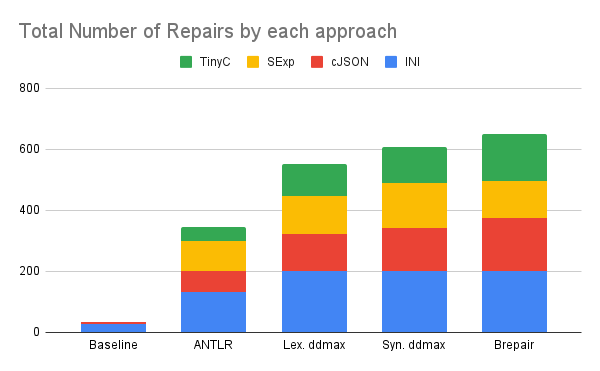
\includegraphics[width=0.45\textwidth]{figures/effectiveness.png}
\pgfplotstableread{
Label      INI    cJSON    SExpParser   TinyC
Baseline   27     6        0            0
ANTLR      133    69       96           46
Lex.ddmax  201    122      124          106
Syn.ddmax  201    140      148          119
BRepair    201    173      122          154
    }\effectivenessdata
\begin{minipage}{.45\textwidth}
\begin{tikzpicture}
\begin{axis}[
    ybar stacked,
    ymin=0,
    ymax=750,
    xtick=data,
    bar width=25,
    legend style={cells={anchor=west}, legend pos=north west},
    reverse legend=true,
    xticklabels from table={\effectivenessdata}{Label},
    xticklabel style={text width=2cm,align=center,font=\footnotesize},
    xtick style={draw=none},
]
    \addplot [fill=darkgray] table [y=INI, meta=Label, x expr=\coordindex] {\effectivenessdata};
    \addlegendentry{INI}
    \addplot [fill=gray] table [y=cJSON, meta=Label, x expr=\coordindex] {\effectivenessdata};
    \addlegendentry{cJSON}
    \addplot [fill=lightgray] table [y=SExpParser, meta=Label, x expr=\coordindex] {\effectivenessdata};
    \addlegendentry{SExpParser}
    \addplot [fill=white,nodes near coords,point meta=y] table [y=TinyC, meta=Label, x expr=\coordindex] {\effectivenessdata};
    \addlegendentry{TinyC}
\end{axis}
\end{tikzpicture}
\end{minipage}
\caption{Number of files repaired by each approach}
\label{fig:effectiveness}
%\vspace{-0.6cm}
\end{figure}

\begin{figure}[!tbp]
\vspace{-0.4cm}
\centering
\begin{minipage}[b]{0.45\textwidth}
    \centering
    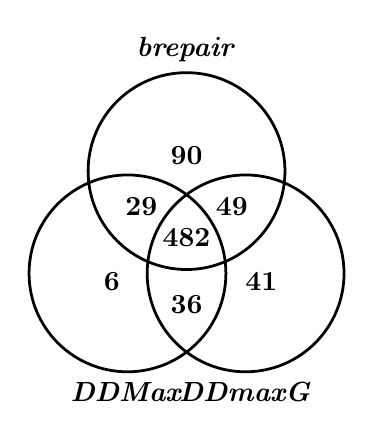
\begin{tikzpicture}[circ/.style={draw=black,line width=1pt,fill=none,shape=circle,minimum width=2.5cm,minimum height=2.5cm},lbl/.style={font=\bfseries}]
        \node[draw=none,minimum width=1.5cm,minimum height=1.29904cm,inner sep=0,outer sep=0] at (0,0) (anchor) {};
        \node[circ] at (anchor.south west) (g1) {};
        \node[circ] at (anchor.south east) (g2) {};
        \node[circ] at (anchor.north) (g3) {};
        \node[lbl,anchor=north] at (g1.south) {\ddmax};
        \node[lbl,anchor=north] at (g2.south) {\ddmaxg};
        \node[lbl,anchor=south] at (g3.north) {\brepair};
        \node[lbl] at ($(g1)!0.5!(g2) - (0,.4)$) {36};
        \node[lbl] at ($(g2)!0.5!(g3) + (.2,.2)$) {49};
        \node[lbl] at ($(g1)!0.5!(g3) + (-.2,.2)$) {29};
        \node[lbl] at ($(anchor.center) - (0,.2)$) {482};
        \node[lbl] at ($(g1.center) - (.2,.1)$) {6};
        \node[lbl] at ($(g2.center) - (-.2,.1)$) {41};
        \node[lbl] at ($(g3.center) + (0,.2)$) {90};
    \end{tikzpicture}
\end{minipage}
%\vspace{-0.4cm}
\caption{Venn Diagram showing the number of invalid inputs repaired (solely) by a (combinations of) technique(s) %, or the combination of approaches
}
\label{fig:repair-complementarity}
\vspace{-0.4cm}
\end{figure}

%\begin{figure}[!tbp]
%\vspace{-0.1cm}
%\centering
%%\includegraphics[width=0.45\textwidth]{images/perfect_bug_understanding}
%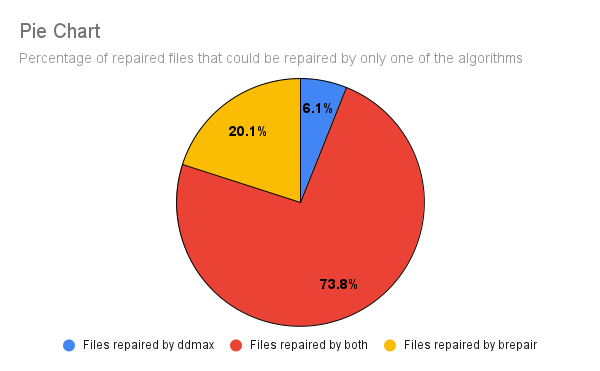
\includegraphics[width=0.5\textwidth]{figures/complementarity_pie_chart.png}
%\vspace{-0.6cm}
%\caption{XXX}
%\label{fig:repair_complementarity}
%\vspace{-0.6cm}
%\end{figure}

\noindent
\textbf{\textit{Contribution of %\approach's 
Input Synthesis:}} We further examine the contribution of input synthesis, i.e., the insertion of input elements to the effectiveness of our approach. This is particularly important since in comparison to ddmax, \approach not only removes invalid input fragments, it also synthesis input elements during repair. 
%To achieve this, 
Using the 321 inputs repaired by all approaches with edit distance data, 
we examine the number of deletion and insertions performed by \approach, this is reported in \autoref{tab:brepair-insertions}. 
% reports the number of deletions and insertions performed by \approach. 

In this experiment, we found that \textit{input synthesis accounts for almost half (49\%) of the repair operations of \approach}. Indeed, \approach performed more insertion operations than deletion operations for two input formats (CJSON and SExp). This result demonstrates the importance of \textit{input synthesis} in comparison to \textit{repairing to subsets}. This demonstrates the advantage of input synthesis via rich failure feedback, and implies that insertion operations are equally as important as deletion operations for effective input repair. 

\begin{result}
Input synthesis is vital to the effectiveness of \approach: Almost half (49\%) of \approach's repair operations are %due to input syntehesis, i.e. 
insertion operations. % of input elements. 
\end{result}


\begin{table}[!tbp]\centering
\caption{Number of edit operations (insertion/deletions) performed by \approach, higher number operations are in \textbf{bold}}
%\vspace{-0.5cm} 
\small
\begin{tabular}{|l | c | r  r  r  r |}
\hline
&  \multicolumn{5}{c|}{\textbf{Number of  Operations}}  \\
\textbf{Ops.} & \textbf{ALL (\%)} & \textbf{INI} & \textbf{cJSON} & \textbf{SExp} & \textbf{TinyC} \\
\hline
\textbf{Insert} & 751 (49\%) & 83 (38\%) &	\textbf{318 (51\%)} &	\textbf{126 (53\%)} &	224 (48\%) \\ 
\textbf{Delete}  & \textbf{794 (51\%)} & \textbf{135 (62\%)} &	308 (49\%) &	110 (52\%) &	\textbf{241 (51\%)} \\ 
\hline
\end{tabular}
\label{tab:brepair-insertions}
%\vspace{-0.5cm}
\end{table}



\noindent \textbf{\textit{Complementarity to Ddmax:}} We further inspect the unique repairs achieved by each approach, in order to understand the complementarity of our approach to the state-of-the-art methods. In this experiment, we inspect the number of unique repairs achieved \textit{solely} by a single approach (e.g., \textit{only} \approach), or two or more approaches (e.g., all approaches).  The goal is to determine if there are unique sets of inputs that are solely repaired by a single approach, and not by other approaches. \autoref{fig:repair-complementarity} and \autoref{tab:repair-complementarity} highlight our findings on the complementarity of \approach to ddmax. 
%to the state-of-the-art.
%demonstrate that our approach complements 
%the complementarity of our approach to 
%DDmax. 

In our evaluation, we found that about 12\% of all repairs could only be completed by \approach, which is is up to 15 times as many as DDmax repairs (\textit{see} \autoref{fig:repair-complementarity}). 
%our 
\approach \textit{solely} repaired more than 
%for %repairs 
\textit{one in every eight} invalid inputs (12\% of repairs), %\approach is the solely repaired them, 
%i.e., 
all of which ddmax could not repair. % these inputs. %. In addition, \approach \textit{solely} repairs 
%which 
%This is up to 15 times as many as DDmax repairs.
\autoref{tab:repair-complementarity} shows that for lexical ddmax, our approach \textit{solely} repaired 15x as many invalid files as lexical ddmax (90 versus six), while it repairs more than twice as many files as syntactic ddmax (90 versus 41). 
% \textit{one in five (20\% of) invalid inputs could be repaired solely by \approach}. \autoref{tab:repair-complementarity} and \autoref{fig:repair-complementarity} highlight the complementarity of \approach to ddmax. 
These findings show that our approach not only outperforms ddmax, but it is also complementary to ddmax: It solely repairs 90 (11\% of all) invalid inputs, all of which ddmax could not repair. %This is evident since it solely completes (12\% of) repairs that could not be completed by the state-of-the-art (ddmax). 
Further 
%experiment 
inspection suggests that this unique repairs achieved by \approach are due to the \textit{rich failure feedback} and \textit{repair via insertion} synergy of \approach. 
%insertion and 

% performance   


\begin{result}
%Our input repair 
\approach 
%not only outperforms the baseline, but 
outperforms and complements the best state-of-the-art method (ddmax).
%\approach 
It is the only technique that can solely complete 12\% of all repairs, which is up to 15 times as many as ddmax. 
\end{result}

\noindent
\textbf{RQ2 Data Recovery and Data Loss:} In this experiment, we investigate the amount of data recovered (and lost) by our approach (\approach). To this end, we compute the file sizes of repaired inputs, and the edit distance between the repaired input and the original input using Levenshtein distance. In addition, we compare the data loss and recovery achieved by our approach to that of the state of the art, i.e. ddmax. 
%For this experiment, we computed the (difference in) files sizes and the Levenshtein distance between the original input and the repaired inputs. 
For a fair evaluation of data recovery, we used 475 inputs that were completely repaired by all three approaches (lexical ddmax, syntactic ddmax and \approach). 
% before a timeout to evaluate data recovery in terms of file sizes.  % and which were completely repaired by all three approaches before a timeout. 
%This resulted in a set of set of (321) inputs for the evaluation of data loss. 


\begin{table}[!tbp]\centering
\caption{Data Recovery of \approach vs. the state-of-the-art}
%\vspace{-0.5cm} 
\begin{tabular}{|l | c | r  r  r  r |}
\hline
&  \multicolumn{5}{c|}{\textbf{\% Data Recovered by Approach}}  \\
&  \multicolumn{1}{c|}{\textbf{ALL}} & \multicolumn{4}{c|}{\textbf{Input Format}}  \\
\textbf{Techniques} & \textbf{Avg. (Tot.)} & \textbf{INI} & \textbf{cJSON} & \textbf{SExp} & \textbf{TinyC} \\
\hline
%\textbf{Baseline}   & (\%) & &  & 	& \\
%\textbf{ANTLR} & (\%) & &  & 	& \\
\textbf{Lex. ddmax} & 86\% (87\%) & \textbf{86.6\%} & 87.1\%	 & 98.5\%	& 70.0\% \\			
\textbf{Syn. ddmax} & 80\% (70\%) & 68.5\% & 83.8\%  & 96.9\%	& 70.6\% \\	
\hline 
\textbf{\approach} & \textbf{ 95\% (88\%)} & \textbf{86.6\%} & \textbf{96.0\%} & \textbf{100.0\%}	& \textbf{97.6\%} \\
\hline
\textbf{Impr. vs. Lex.} & \textbf{13\%} (1\%) & 0.1\%	& \textbf{10.2\%}	& 1.5\%	& \textbf{39.4\%} \\
\textbf{Impr. vs. Syn.} & \textbf{21\% (25\%)} & \textbf{26.5\%} 	& \textbf{14.5\%}	& 3.1\%	& \textbf{38.2\% }\\
\hline
%\textbf{Total \#Repairs} & (\%) & &  & 	& \\		
%\hline
\end{tabular}
\label{tab:data-recovery}
%\vspace{-0.5cm}
\end{table}

\noindent
\textbf{\textit{Data Recovery:}} \autoref{tab:data-recovery} and \recheck{Figure X} illustrate the data %loss and data 
recovery achieved by each approach. %Our evaluation r
Results show that \textit{\approach recovered up to 88\% of input data and which is up to 25\% more than the most effective baseline (syntactic ddmax).} %Notably, f
For all four input formats, \approach recovered more data than the both variants of ddmax. As an example, for TinyC, \approach recovered about 39\% more input data than the state-of-the-art. 
Overall, this result suggests that \approach is more effective in recovering valid input data than ddmax. 

\noindent
\textbf{\textit{Data Loss:}} To measure data loss, we compute the Levenshtein distance between repaired and invalid files using %Meanwhile, %For a balanced and tractable evaluation of data loss, 
%we employed the 
a set of 321 completely repaired inputs %by all three approaches which %(321) inputs that 
%which the Levenshtein distance implementation could compute %their edit distance 
where edit distance could be computed within a threshold of 750 edit distances (about 30 seconds). 

We found that \textit{\approach achieves a low data loss of about 13 edit distances,on avarage},  which is \textit{up to 23 times lower than (lexical) ddmax}. \autoref{tab:data-loss} shows this result of this experiment. For almost all input formats, \approach achieved a lower data loss than syntactic and lexical ddmaz (except for INI and SExp). This performance is attributed to the rich fasilure feedback of \approach, which allows it to distinguish between incomplete and incorrect input fragments. 

\begin{result}
\approach has a high data recovery rate (98\%, on average) and its data %The data recovery and 
loss is up to 23 times lower than that of ddmax (e.g., INI).     
\end{result}


\begin{table}[!tbp]\centering
\caption{Data Loss (Levenshtein distance) of \approach vs. the state-of-the-art (ddmax), minimum data loss and significant \% reduction in data loss are in \textbf{bold}}
%\vspace{-0.5cm} 
\begin{tabular}{|l | c | r  r  r  r |}
\hline
&  \multicolumn{5}{c|}{\textbf{Average Data Loss }}  \\
\textbf{Techniques} & \textbf{ALL} & \textbf{INI} & \textbf{cJSON} & \textbf{SExp} & \textbf{TinyC} \\
\hline
\textbf{Lex. ddmax} & 17.5 & \textbf{10.2} &	56.5 &	\textbf{6.6} &	 8.4 \\	
\textbf{Syn. ddmax} & 119.6 &  258.1 & 76.6 &	75.2 &	30.6 \\
\textbf{\approach} & \textbf{13.0}  & 11.2 &	\textbf{35.0} &	7.3 & \textbf{4.0} \\
\hline
\textbf{\% Reduc. vs. Lex.} & \textbf{35\%} &  -9\% & \textbf{61\%} & -9\% & \textbf{108\%} \\
\textbf{\% Reduc. vs. Syn.} & \textbf{818\%} & \textbf{2195\%} &	\textbf{119\%} & \textbf{936\%} &\textbf{ 656\%} \\
\hline
\end{tabular}
\label{tab:data-loss}
%\vspace{-0.5cm}
\end{table}


\noindent
\textbf{RQ3 Diagnostic Quality:} 
In this experiment, we evaluate the diagnostic quality of \approach in comparison to the state-of-the-art techniques. In particular, we compare the size of the diagnoses, i.e., the isolated failure cause reported by each approach, as well as the intersection of the diagnoses reported by these approaches. We compare \approach to three main methods, namely \approach, lexical ddmax, syntactic ddmax and ddmin.  \recheck{Table x and figure X} show the diagnostic quality of our approach, in comparison to the state of the art techniques. 

We found that 

\begin{result}
XXXX
XXXX
\end{result}





\noindent
\textbf{RQ4 Efficiency:}
%\todo{mention that run-time is the execution time of the algorithm, without accounting for the time for experimental pre/post processings }
Let us evaluate the performance of our approach. 
%, i.e., %we investigate 
%how long it takes \approach to repair an invalid input, in comparison to the state-of-the-art (ddmax). 
%In addition, w
%We also evaluate the number %of repair attempts, i.e., number of 
%program runs %test experiments with input fragments, 
%performed by each approach. 
To this end, we measure the time performance (i.e., execution time) and the number of program runs performed 
%  of input repairs that were completed 
by \approach, in comparison to lexical ddmax and syntactic ddmax. For a balanced evaluation, we 
%performed an experiment analysing % where we consider %for 
analyse a set of 483 invalid inputs % files 
that where completely repaired by all three approaches within %, in less than 
two minutes, %. % (120,000ms). 
%Specifically
%To be fair, we report the execution time of each algorithm, 
without %accounting for 
%the time for 
data collection and % or experimental 
analysis time. 
%For program runs, w
%We also compute the number of program runs, i.e., %repair attempts, 
%the number of program execution during the test experiments of each approach.  
%\recheck{
\autoref{tab:efficiency} %and figure X} 
illustrates the efficiency of our approach compared to ddmax. %the state-of-the-art methods. 

%For runtime, 

In this evaluation, we found that \textit{\approach is efficient in input repair: It is reasonably fast, it takes about \recheck{1.7} seconds to repair an invalid input file, on average}. 
\approach is 50\% more efficient than lexical ddmax (\recheck{1.7s versus 2.5s}), and syntactic ddmax is about three times as efficient as \approach (\recheck{0.6s versus 1.7s}). 
%The time performance of 
%This implies that \approach is twice as fast as %er than 
%lexical ddmax, but twice slower than syntactic ddmax. 
This result is %ese findings are 
due to the %can be explained 
% is expected since the execution time of %repair attempts (i.e., 
%by the 
number of program runs required by each approach. 
%, which is  %) 
%the main time-consuming component of \approach, as well as ddmax. 
%However,
%\recheck{
\autoref{tab:efficiency} %} %  and Table/Figure X show} 
shows %the %Inspecting 
the number of %repair attempts (aka 
program runs performed by each approach. %for all approaches.
For instance, the execution time 
%performance cost is much lower for 
of \approach %syntactic ddmax 
is much higher %lower 
than that of syntactic ddmax 
%and \approach, since 
because \approach requires about three times as many program runs as syntactic ddmax (\recheck{505 vs. 1,586} program runs). 
%these approaches is the number of repair attempts and both lexical ddmax and \approach perform more test experiments than syntactic ddmax, 
The lower program runs required by syntactic ddmax is because %since 
it leverages the input grammar to reduce the number of test experiments. 
%, i.e. test experiments with input fragments. 
% %) 
%It shows that \approach performed \recheck{X} less repair attempts than lexical ddmax (\recheck{X vs. X} runs), and 
%\recheck{X} as many repair attempts as lexical ddmax (\recheck{X vs. X} runs). 
%We observe that 
Overall, %these results suggest that 
\approach is reasonably efficient, and %it is 
more efficient than lexical ddmax. %In addition, w
We observe that the number of program runs is the main performance bottleneck of all three approaches. % to the 
%These results suggest that \approach is %not very time-consuming or 
%inexpensive, it as a reasonable number of repair attempts and time performance, especially in  comparison to lexical ddmax. 

\begin{result}
%Our 
\approach %is %reasonably fast, 
%it 
repairs an invalid input in less than \recheck{two} (1.7) seconds, on average. %\approach 
It is 50\% more effective than lexical ddmax, but 2x slower than syntactic ddmax. 
% is three times as %effective as %only half as 
%fast 
%syntactic ddmax. 
\end{result}

\begin{table}[!tbp]\centering
\caption{Efficiency of \approach vs. the state-of-the-art (ddmax), lower runtime, smaller number of program runs %and significant \% improvement in efficiency 
are in \textbf{bold}, second-best time performance is in \textit{italics}}
%\vspace{-0.5cm} 
\begin{tabular}{|l |  r  r | r  r |}
\hline
%& \textbf{\#Repaired} 
&  \multicolumn{2}{c|}{\textbf{Runtime (s)}} & \multicolumn{2}{c|}{\textbf{\#Prog. Runs}}  \\
\textbf{Techniques} %& \textbf{Inputs} 
&  \textbf{Avg.}  & \textbf{Total} & \textbf{Avg.}  & \textbf{Total} \\
\hline
\textbf{Lex. ddmax} & %483 & 
2.5 & 1188 & 2084 & 1006682 \\
\textbf{Syn. ddmax} & %483 & 
\textbf{0.6} & \textbf{280}  & \textbf{505}  & \textbf{244022}  \\
\hline
\textbf{\approach} &  %483 & 
\textit{1.7} & \textit{845}  & \textit{1586} & \textit{765987}  \\
\hline
%\textbf{\approach vs. Lex.} &  & & & \\
%\textbf{\approach vs. Syn.} & & & & \\
%\hline
\end{tabular}
\label{tab:efficiency}
%\vspace{-0.5cm}
\end{table}




%\noindent
%\textbf{RQ4 Comparison to the state-of-the-art:} 
%
%
%\noindent \textit{ Effectiveness \& Efficiency:}
%\begin{result}
%
%\end{result}
%%
%%\noindent \textit{Efficiency:}
%%\begin{result}
%%
%%\end{result}
%
%\noindent \textit{Data Recovery \& Loss:}
%
%\begin{result}
%
%\end{result}
%
%\noindent \textit{Diagnostic Quality:}
%
%\begin{result}
%
%\end{result}



\section{Discussion}

\section{Threats to Validity}

\todo{discuss threats to validity .... discuss issues like input synthesis (insertion), requires rich feedback: incorrect and incomplete input fragment}
Our approach (\approach) and empirical evaluations may be limited by the following validity threats:

\noindent
\textbf{External Validity:}

\noindent
\textbf{Internal Validity:}


\noindent
\textbf{Construct Validity:}


\section{Related Work}
\label{sec:related_work}
%TODO In this chapter, we discuss...

\todo{refactor this section, looks to similar to ddmax, also add Infix paper ... }

%\begin{description}

\noindent
\textbf{Input Rectification} is the process of transforming misbehaving inputs into inputs that behave predictably in the scope of a certain software system.
    In \textit{Automatic Input Rectification}~\cite{Long:2012:AIR:2337223.2337233} and \emph{Living in the Comfort Zone}~\cite{Rinard:2007:LCZ:1297027.1297072}, input constraints are learned from valid inputs to solve this problem, which are used to transform malicious inputs into rectified inputs that satisfy learned constraints.
    We do not employ such constraint learning techniques in \bfr.
    Instead, we employ the knowledge of a grammar describing the input file format and the feedback of a subject program to transform the input files into an acceptable subset.
    Instead of transforming inputs to comply to security-critical constraints, our goal is to recover as much of the input file as possible.

\noindent
\textbf{File Recovery} aims to recover files that cannot be opened with a subject program due to corruption.
In \emph{S-DAGs}~\cite{scheffczyk2004s}, semantic consistency constraints are enforced on broken input files in a semi-automatic technique.
\emph{Docovery}~\cite{docovery:ase14} takes a similar approach using symbolic execution to change broken inputs to take error-free paths in the subject program.
While this is a whitebox approach that facilitates program analysis, \bfr relies on the feedback of the subject program in a black-box approach that results from executing the broken inputs.

\noindent
\textbf{Input Debugging}, in contrast to program debugging, aims to change inputs to localize faults in subject programs.
    There is numerous work that focuses on simplifying failure-inducing inputs~\cite{zeller2002simplifying, clause2009penumbra, hierarchicalDD, sterling2007automated}.
    Closely related to \bfr are particularly \cite{hierarchicalDD} and \cite{sterling2007automated}, which both aim to minimize the input files while still triggering a bug in the subject program, just like \ddmin.
    In contrast, \bfr tries to maximize the inputs while avoiding to trigger the bug in the subject program.

\noindent
\textbf{Data Diversity} \cite{data_diversity} transforms a failure-inducing input into an input that can be processed by a subject program while generating the same output.
Their approach analyzes which regions of the input cause the fault and changes those regions to avoid the fault.
An important difference to \bfr is that we do not need any program analysis, but analyze the output of the subject program alone.

\noindent
\textbf{Data Structure Repair} iteratively fixes corrupted data structures by enforcing they conform to consistency constraints~\cite{Demsky:2003:ADR:949343.949314, 1553560, hussain2010dynamic, Demsky:2006:IED:1146238.1146266}.
These constraints can be extracted, specified and enforced with predicates~\cite{elkarablieh2008juzi}, model-based systems~\cite{Demsky:2003:ADR:949343.949314}, goal-directed reasoning~\cite{1553560}, dynamic symbolic execution~\cite{hussain2010dynamic} or invariants~\cite{Demsky:2006:IED:1146238.1146266}.
Similarly to our approach, one goal in data structure repair is to successfully execute a subject program on broken input files safely and acceptably.
However, \bfr focuses on repairing inputs while recovering as much data as possible to avoid inducing faults in the subject program.

\noindent
\textbf{Syntactic Error Recovery} is the implementation of error recovery schemes, typically in parsers and compilers~\cite{hammond1984survey, backhouse1979syntax}.
In most of the syntactic recovery approaches, various different techniques are employed, including insertion, deletion and replacement of symbols~\cite{anderson1981locally, cerecke2003locally, anderson1983assessment}, extending forward or backwards from a parser error~\cite{burke1982practical, mauney1982forward}, or more general methods of recovery and diagnosis~\cite{krawczyk1980error, aho1972minimum}.
Different to \bfr, these schemes ensure the compiler does not halt while parsing, while our approach aims to fix the input inducing the failure.

\noindent
\textbf{Data Cleaning and Repair} is typically performed on complex database systems.
In most approaches, this includes analyzing the database to remove noisy data or fill in missing data~\cite{xiong2006enhancing, hernandez1995merge}.
In other approaches, developers are allowed to write and apply logical rules on the database~\cite{pochampally2014fusing, galhardas2000ajax, golab2010data, jeffery2006pipelined, raman2001potter, luebbers2003systematic}.
While all of these approaches repair database systems, \bfr repairs raw user inputs.

\noindent
\textbf{Data Testing and Debugging} aims to identify program errors caused by well-formed but incorrect data while a user modifies a database~\cite{mucslu2013data}.
In continuous data testing (CDT)~\cite{mucslu2015preventing}, likely data errors are identified by continuously executing domain-specfic test queries, in order to warn users of test failures.
\emph{DATAXRAY}~\cite{wang2015error} also investigates the underlying conditions that cause data bugs, it reveals hidden connections and common properties among data errors.
In contrast to \bfr, these approaches aim to guard data from new errors by detecting data errors in database systems during modification.
%\end{description}

\section{Conclusion}
\todo{discuss potential future works}

\revise{We provide our tool, data and experimental results for easy replication, scrutiny and reuse:
}

 \begin{center}
 \vspace{-0.2mm}
     \textbf{\url{https://github.com/XXX}}
 \end{center}
 
% \begin{acks}
% % To Robert, for the bagels and explaining CMYK and color spaces.
% \end{acks}

%%
%% The next two lines define the bibliography style to be used, and
%% the bibliography file.
\bibliographystyle{ACM-Reference-Format}
\bibliography{fse22-brepair}


\end{document}
